\section{Anwendung und Grundlage der uP-Technik}
\begin{multicols}{2}
\subsection{Anwendungen}
\begin{minipage}{5cm}
\begin{itemize}
    \item Supercomputer
    \item Arbeits und Server-Rechnern
    \item Smartphones
    \item Navigationssysteme
    \item Digitalkameras
    \item Drucker
    \item ...
\end{itemize}
\end{minipage}

\subsection{Aufbau}

Verstehe die wesentlichen System-komponetnen des Rechnersystems auf einem IC (Integrated Circuit)\\	
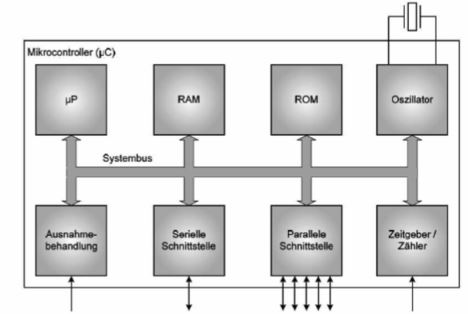
\includegraphics[width=7cm]{images/aufbauuC}

\end{multicols}
\subsubsection{Aufbau uP-basierten Systeme}
\begin{itemize}
    \item Zentraleinheit CPU mit
    \begin{itemize}
        \item Rechenwerk ALU
        \item Steuerwerk CU
    \end{itemize}
    \item Speicher
    \item \textbf{Eingabe-/Ausgabe-}Schnittsellen
\end{itemize}
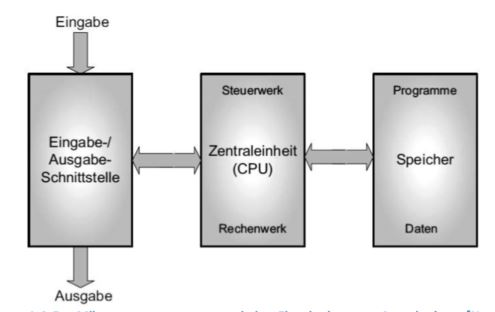
\includegraphics[width=7cm]{images/aufbauuC1}
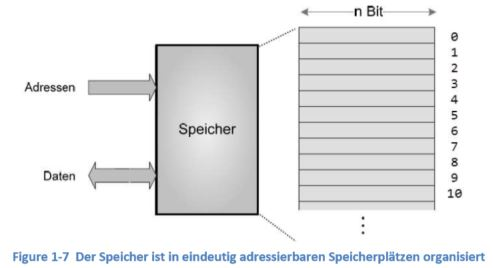
\includegraphics[width=7cm]{images/aufbauuCspeicher}

\subsubsection{Havard vs Von Neumann Architektur}
\begin{multicols}{2}
    \textbf{Harvard Rechnermodell}\\
    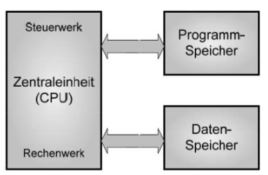
\includegraphics[width=7cm]{images/HavardArchi}
    \\	
    \textbf{von Neumann Rechnermodell}\\
    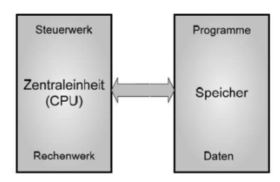
\includegraphics[width=7cm]{images/NeumannArchi}
\end{multicols}

\subsubsection{Programmierung eins uP}
\begin{minipage}{10cm}
    Ein \mu P kann durch individuelle Programmierung auf ganz unterschiedliche Art angepasst werden. \newline
    \rightarrow entscheidend für die Durchdrinngung im Markt.\newline
    Ein Programm enthält in aufeinanderfolgender Anordnung die Maschinen-Befehle oder -Instruktionen für den \mu P. Diese Maschiene-Befehle teilen der CPU mit, welche Operationen in welcher Reihenfolge und auf welche Daten angewendet werden sollen, \newline
    Die Befehlsfolge des Programms wird innerhalb der CPU vom Steuerwerk gesteuert und schrittweise ausgeführt. Dazu wird der aktuell zur bearbeitende Befehl durch einen Programmzähler(PC) im Speicher adressiert.\newline
    Der PC enthält laufend die Adresse der Speicherzelle des jeweiligen Befehls im Speicher.
\end{minipage}
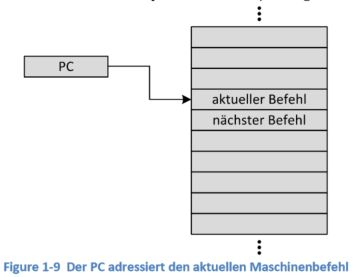
\includegraphics[width=7cm]{images/uPPC}
    
\subsubsection{Befehlsformate}
Die Art und Wirkung eines Befehls wird im Befehlswort(\textbf{OpCode}) codiert \newline
Darin sind neben der Operation auch die Operanden spezifiziert.\\
Die Codierung des Befehlswortes erfolgt abhängig vom \mu P.\\
Der Maschinencode setzt sich aus einem OpCode und einem oder mehreren Operanden zusammen.\\
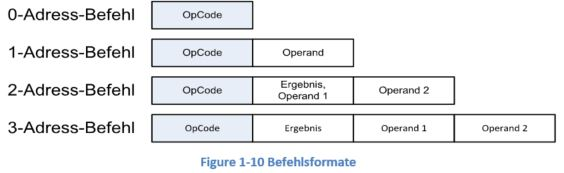
\includegraphics[width=7cm]{images/Befehlsformate}


\subsection{RISC vs CISC}
\begin{multicols}{2}
    \textbf{CISC}\newline
    Complex Instruction Set Computer
    \\
    \textbf{RISC}\newline
    Reduced Instruction Set Computer
\end{multicols}
\subsubsection{RISC-Rechner}
effizienter als CISC-Rechner
\begin{itemize}
    \item besteht aus einer kleien Anz. von Befehlen mit wenigen Adressierungsarten
    \item Registersatz enthält eine grosse Anzahl von allg. verwendbaren Registern\newline
    General Purpose Register (GPR)
    \item Speicherzugriff erfolgt über spezielle Lade- und Speicher-Befehle
    \begin{itemize}
        \item Arithmetische-logische Operationen arbeiten auf Registeroperanden
    \end{itemize}
    \item Pipline-Architecture \leftarrow Leistungssteigernde Architektur
    \item Grosse semantische Lücke entsteht bei der Übersetzung aus der Hochsprache
\end{itemize}

\subsubsection{u Architektur}
Beschriebt die architektonischen Details bei der Implementierung der \mu P aus sicht der Programmierer.
Dies umfassst die Beschreibung der Zentraleinheit (CPU), des Rechenwerks (ALU) und des Steuerwerks (CU).

\subsubsection{Hardware- /Software-Schnitsttelle}
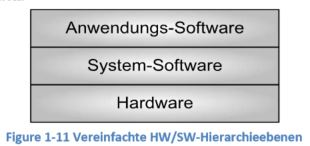
\includegraphics{images/HardwareSoftware}
\subsubsection{Hardware}
\textbf{Registersatz}\newline
Register sind schnelle Zwischenspeicher für temporäre Daten im \mu P.\\

\textbf{Taktfrequenz}\newline
Das Taktsignal steuert die zeitliche Abfolge im \mu P \newline

\[ f_{Takt}= \frac{1}{T_{takt}} \]
$ \Uparrow $ Taktrate $ \Leftrightarrow $$  \Uparrow  $Leistungsaufnahme \\
Um Energie zu sparen ist es sinnvoll die Taktrate laufend anzupassen.\\

\textbf{Leistungsaufnahme}
\begin{multicols}{2}
\[ P_{Gate}= \frac{1}{2} \cdot C_{Last} \cdot V_{DD}^2\cdot f_{Takt} \]\\
$ P_{Gate} \qquad$Leistung pro CMOS Gate \newline
$ C_{Last} \qquad $Lastkapazität\newline
$ V_{DD}\qquad $Versorgungsspannung\newline
$ f_{Takt} \qquad$Taktfrequenz
\end{multicols}

\subsubsection{Software}
\begin{multicols}{2}
\textbf{Ablauf}\newline
\begin{itemize}
    \item Der Präprozessor bereitet das Quellprogramm für den Compiler vor
    \item Der Compiler übersetz das Programm von einer Hochsprache in Assembly-Programm
    \item Der Binder fasst verschiedene Dateien, die verschiebbaren Maschinencode enthalten zu einem Programm zusammen.
    \item Der Loader wandelt die verschiebbaren Adressen in Absolute Adressen um und läd sie in den Speicher des Systems.
\end{itemize}

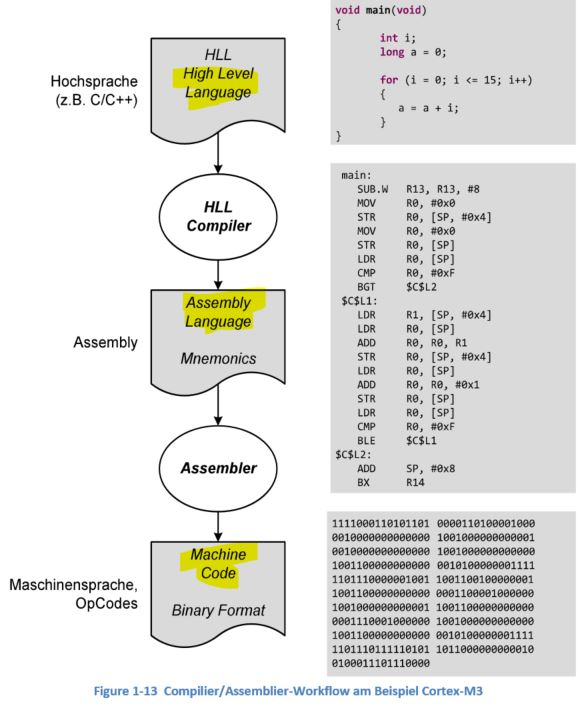
\includegraphics{images/CompilerWorkflow}
\end{multicols}

\subsubsection{Compiler-Schritte}
\begin{multicols}{2}
    \begin{itemize}
        \item \textbf{Lexikalische Analyse(scanning):}\newline
        Die Symbole der Sprache werden erkannt und Gruppiert. Leerzeichen werden eliminiert
        \item \textbf{Syntaxanalyse(parsing):} Die erlannten Symbole werden in Sätzen zusammengefasst und in einem Parsbaum dargestellt
        \item \textbf{Semantische Analyse:} Das Quellprogramm wird auf Fehler überprüft( zBsp. Typfehler) und der Parsbaum erhält Informationen über die verwendeten Bezeichner
        \item \textbf{Zwischencode-Erzeugung:} Einige COmpiler erzeugen Code in einer Zwischensprache (abstrakte Maschinen)
        \item \textbf{Code-Erzeugung:} Erzeugen von verschiebbarem Maschinencode.      
    \end{itemize}

    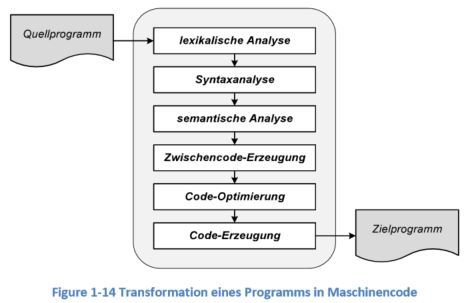
\includegraphics[height=7.5cm]{images/CompilerWorkflow2}
\end{multicols}

\subsubsection{Busortientierte Systeme}
\textbf{Speicher}
\begin{multicols}{2}
    \textbf{RAM}
    \begin{itemize}
        \item Random Access Memory
        \item Schreibe-/Lese-Speicher
        \item Spannungsversorgung erforderlich
        \item für Temporär Daten
    \end{itemize}

    \textbf{ROM}
    \begin{itemize}
        \item Read Only Memory
        \item Festwert Speicher
        \item auch ohne Spg. bleiben Daten erhalten
    \end{itemize}
\end{multicols}

\begin{multicols}{3}
\begin{minipage}{4cm}
        \textbf{Adressbus}
    \begin{itemize}
        \item unidirektional
        \item bestimmt Grösse des Adressraums
    \end{itemize}
\end{minipage}

\begin{minipage}{4cm}
    \textbf{Databus}
    \begin{itemize}
        \item bidirektional
    \end{itemize}
\end{minipage}

\begin{minipage}{5cm}
    \textbf{Steuerbus}
    \begin{itemize}
        \item kontrolliert Buszugriffe
        \item zeitlicher Ablauf der Signale
    \end{itemize}
\end{minipage}
\end{multicols}

\begin{itemize}
    \item Die gesammte Menge der über den Adressbus adressierbaren Speicherzellen wird \textbf{Adressraum} genannt
    \item Die Anzahl parallel geführten \textbf{Datenleitungen} entspricht der maximal zu übertragenden Datenbreite
    \item Kontrollsigbale werden über den \textbf{Steuerbus} übertragen
\end{itemize}
    \includegraphics[height=7.5cm]{images/SimpleuPSystem}
    
\subsubsection{Architectur eines uP}
    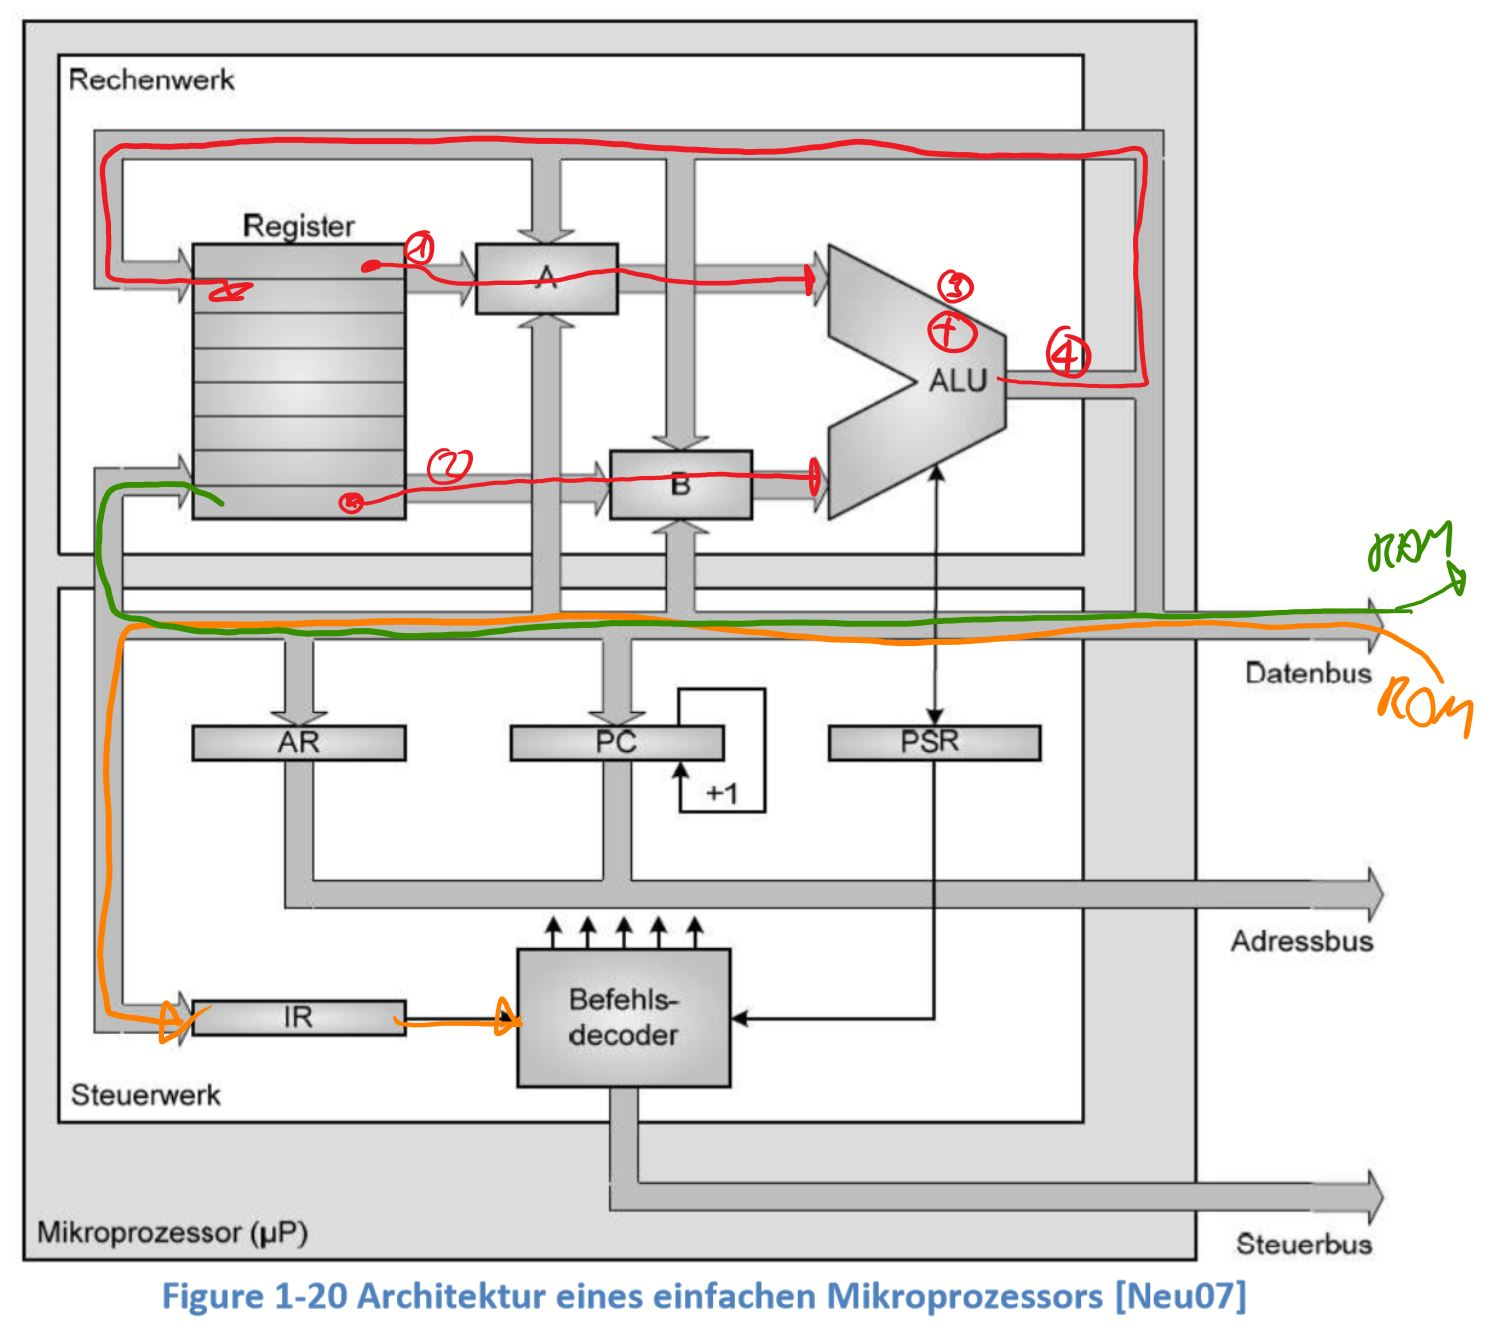
\includegraphics[height=7.5cm]{images/ArchitectuP}\\
    
\begin{multicols}{2}
\begin{minipage}{8cm}
\textbf{Flags}\newline
\begin{tabular}{|c|c|l|}
    \hline 
    \textbf{N}  & \textbf{Negative} & Das von der ALU berechnete Ergebniss ist negativ \\ 
    \hline 
    \textbf{Z}  & \textbf{Zero} & Das von der ALU berechnete Ergenis ist gleich \textbf{0} \\ 
    \hline 
    \textbf{C}  &\textbf{Carry}  &Die Berechnung der ALU hat zu einem Übertrag geführt  \\ 
    \hline 
    \textbf{V}  &\textbf{Overflow}  & Die Berechnung der ALU hat zu einem Overflow geführt  \\ 
    \hline 
\end{tabular} 
\end{minipage}

\begin{minipage}{5cm}
    \begin{tabular}{c|c}
        \textbf{AR}&Adressregister  \\ 
        \textbf{PC}&Programm Counter  \\ 
        \textbf{PSR}& Program Status Register \\ 
        \textbf{IR}& Instruction Register  \\ 
    \end{tabular} 
\end{minipage}
\end{multicols}

\subsection{Befehlszyklus}
    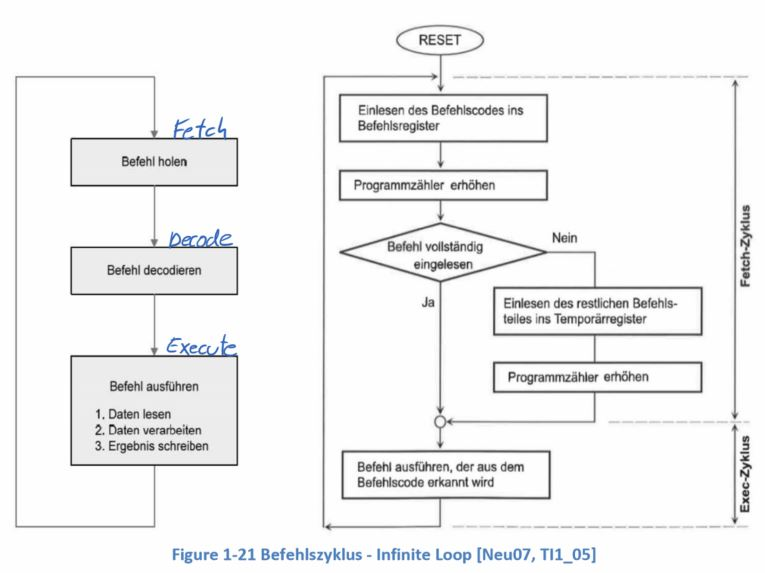
\includegraphics[height=9cm]{images/CommandFlowChart}





















    